%
% lines.tex
%
\renewcommand{\thisname}{Chart::Lines}
\section{\thisname}
\name{\thisname}
\requires{Chart::Base, GD, Carp, FileHandle}
\begin{Description}
The class \thisclass creates a lines chart. (If you want the data
points marked with symbols, check \class{Chart::LinesPoints} on
page \pageref{Chart::LinesPoints}.) \thisclass is a subclass of
\class{Chart::Base}.
\end{Description}

\example
\begin{figure}[ht]
  \begin{center}
    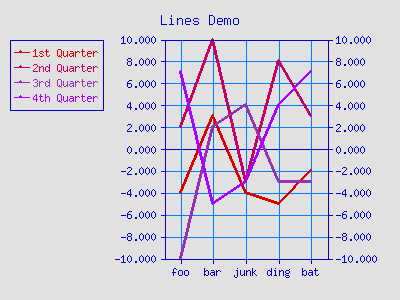
\includegraphics[scale=0.5]{d_lines2.png}
  \end{center}
  \caption{Lines chart}
  \label{fig:lines}
\end{figure}
\begin{verbatim}
use Chart::Lines;

$g = Chart::Lines->new();
$g->add_dataset('foo', 'bar', 'junk', 'ding', 'bat');
$g->add_dataset( -4,  3, -4, -5, -2);
$g->add_dataset(  2, 10, -3,  8,  3);
$g->add_dataset(-10,  2,  4, -3, -3);
$g->add_dataset(  7, -5, -3,  4,  7);

%hash = ('legend_labels' => ['1st Quarter', '2nd Quarter',
                             '3rd Quarter', '4th Quarter'],
         'y_axes'              => 'both',
         'title'               => 'Lines Demo',
         'grid_lines'          => 'true',
         'legend'              => 'left',
         'legend_example_size' => 20,
         'colors' => {'text'       => 'blue',
                      'misc'       => 'blue',
                      'background' => 'grey',
                      'grid_lines' => 'light_blue',
                      'dataset0'   => [220,0,0],
                      'dataset1'   => [200,0,100],
                      'dataset2'   => [150,50,175],
                      'dataset3'   => [170,0,255]
                     }
        );

$g->set(%hash);

$g->png("lines.png");
\end{verbatim}

\constructorblurb{\thisname}

\begin{AttrDecl}{brush\_size}
Sets the width of the lines in pixels. Default is 6.
\end{AttrDecl}

\begin{AttrDecl}{sort}
Sorts the data in ascending order if set to \literal{true}. Should be
set if the input data is not sorted. Defaults to \literal{false}.
\end{AttrDecl}

\begin{AttrDecl}{stepline}
The points are connected by a stepping function,instead of by a direct
line if set to \literal{true}. Defaults to \literal{false}.
\end{AttrDecl}

\begin{AttrDecl}{stepline\_mode}
Determines whether to plot each stepping line at the level of the
start of the interval (if set to \literal{begin}) or at its end if set
to \literal{end}. Defaults to \literal{begin}.
\end{AttrDecl}

\attrdecl{xlabels}
\begin{AttrDecl}{xrange}
This pair of options allows arbitrary positioning of $x$ axis labels.
The two options must either both be specified or both be omitted.
\attruse{xlabels} is a reference to 2-element array. The first of the
elements is a nested (reference to an) array of strings that are the
labels. The second element is a nested (reference to an) array of
numbers that are the $x$ values at which the labels should be placed.
\attruse{xrange} is a 2-element array specifying the minimum and maximum
$x$ values on the axis. \Eg,
\begin{verbatim}
@labels = (['Jan', 'Feb', 'Mar'],
           [10,    40,    70   ]);
$chart->set(xlabels => \bs @labels,
            xrange  => [0, 100]
           );
\end{verbatim}
\end{AttrDecl}

\begin{AttrDecl}{xy\_plot}
Forces \thisclass to plot a $x$--$y$ graph if set to \literal{true},
\ie, to treat the $x$ axis as numeric. Very useful for plots of
mathematical functions. Defaults to \literal{false}.
\end{AttrDecl}

